\documentclass{article}

\usepackage{tcolorbox}
\usepackage{ulem} %math
\usepackage{amsmath}
\usepackage{amsfonts}
\usepackage{amssymb}
\usepackage{graphicx}
\usepackage{enumerate}


%Create a box for theorems
%\begin{theo}[titel] %optional
%tekst
%\end{theo}
\newenvironment{theo}[1][Vigtigt]{%
\begin{tcolorbox}[colback=green!5,colframe=green!40!black,title=\textbf{#1}]
}{%
\end{tcolorbox}
}




%Create a square matrix
%\begin{ArgMat}{2}
%21 & 22 & 23 \\  
%a & b & c
%\end{ArgMat}
%
% Info: http://tex.stackexchange.com/questions/2233/whats-the-best-way-make-an-augmented-coefficient-matrix
%
\newenvironment{ArgMat}{%
$
  \left[\begin{array}{@{}*{100}{r}r@{}}
}{%
  \end{array}\right]
  $
}

\newenvironment{deter}{%
$
  \left|\begin{array}{@{}*{100}{r}r@{}}
}{%
  \end{array}\right|
  $
}


%Create multiple lines with holes
%\begin{SysEqu}
%x_1 && &- &5x_3 &+ &2x_4=& 1 \\
%x_1 &+ &x_2 &+ &x_3 && =& 4 \\
%&&&&&&0 =& 0
%\end{SysEqu}
\newenvironment{SysEqu}{%
$  \setlength\arraycolsep{0.1em}
  \begin{array}{@{}*{100}{r}r@{}}
}{%
  \end{array}$
}

%Create solution for x_1, x_n...
%\begin{solu}
%x_1 &= d \\
%x_2 &= e \\
%x_3 &= s
%\end{solu}
\newenvironment{solu}{%
$
  \setlength\arraycolsep{0.1em}
  \left\{\begin{array}{@{}*{100}{r}r@{}}
}{%
  \end{array}\right.
$
}

\usepackage{lastpage}


\newcommand{\HRule}{\rule{\linewidth}{0.8mm}}

%Tekst i fotter
\newcommand{\footerText}{\thepage\xspace /\pageref{LastPage}}
\newcommand{\ProjectName}{433 MHz styring af AeroQuad}


\chapterstyle{hangnum}




\nouppercaseheads
\makepagestyle{mystyle} 

\makeevenhead{mystyle}{}{\\ \leftmark}{} 
\makeoddhead{mystyle}{}{\\ \leftmark}{} 
\makeevenfoot{mystyle}{}{\footerText}{} 
\makeoddfoot{mystyle}{}{\footerText}{} 
\makeatletter
\makepsmarks{mystyle}{% Overskriften på sidehovedet
  \createmark{chapter}{left}{shownumber}{\@chapapp\ }{.\ }} 
\makeatother
\makefootrule{mystyle}{\textwidth}{\normalrulethickness}{0.4pt}
\makeheadrule{mystyle}{\textwidth}{\normalrulethickness}

\makepagestyle{plain}
\makeevenhead{plain}{}{}{}
\makeoddhead{plain}{}{}{}
\makeevenfoot{plain}{}{\footerText}{}
\makeoddfoot{plain}{}{\footerText}{}
\makefootrule{plain}{\textwidth}{\normalrulethickness}{0.4pt}

\pagestyle{mystyle}

%%----------------------------------------------------------------------
%
%%Redefining chapter style
%%\renewcommand\chapterheadstart{\vspace*{\beforechapskip}}
%\renewcommand\chapterheadstart{\vspace*{10pt}}
%\renewcommand\printchaptername{\chapnamefont }%\@chapapp}
%\renewcommand\chapternamenum{\space}
%\renewcommand\printchapternum{\chapnumfont \thechapter}
%\renewcommand\afterchapternum{\space: }%\par\nobreak\vskip \midchapskip}
%\renewcommand\printchapternonum{}
%\renewcommand\printchaptertitle[1]{\chaptitlefont #1}
\setlength{\beforechapskip}{0pt} 
\setlength{\afterchapskip}{0pt} 
%\setlength{\voffset}{0pt} 
\setlength{\headsep}{25pt}
%\setlength{\topmargin}{35pt}
%%\setlength{\headheight}{102pt}
%\setlength{\textheight}{302pt}
\renewcommand\afterchaptertitle{\par\nobreak\vskip \afterchapskip}
%%----------------------------------------------------------------------




%Sidehoved og -fod pakke
%Margin
\usepackage[left=2cm,right=2cm,top=2.5cm,bottom=2cm]{geometry}
\usepackage{lastpage}



%%URL kommandoer og sidetal farve
%%Kaldes med \url{www...}
%\usepackage{color} %Skal også bruges
\usepackage{hyperref}
\hypersetup{ 
	colorlinks	= true, 	% false: boxed links; true: colored links
    urlcolor	= blue,		% color of external links
    linkcolor	= black, 	% color of page numbers
    citecolor	= blue,
}



%Mellemrum mellem linjerne    
\linespread{1.5}


%Seperated files
%--------------------------------------------------
%Opret filer således:
%\documentclass[Navn-på-hovedfil]{subfiles}
%\begin{document}
% Indmad
%\end{document}
%
% I hovedfil inkluderes således:
% \subfile{navn-på-subfil}
%--------------------------------------------------
\usepackage{subfiles}

%Prevent wierd placement of figures
%\usepackage[section]{placeins}

%Standard sti at søge efter billeder
%--------------------------------------------------
%\begin{figure}[hbtp]
%\centering
%\includegraphics[scale=1]{filnavn-for-png}
%\caption{Titel}
%\label{fig:referenceNavn}
%\end{figure}
%--------------------------------------------------
\usepackage{graphicx}
\usepackage{subcaption}
\usepackage{float}
\graphicspath{{../Figures/}}

%Speciel skrift for enkelt linje kode
%--------------------------------------------------
%Udskriver med fonten 'Courier'
%Mere info her: http://tex.stackexchange.com/questions/25249/how-do-i-use-a-particular-font-for-a-small-section-of-text-in-my-document
%Eksempel: Funktionen \code{void Hello()} giver et output
%--------------------------------------------------
\newcommand{\code}[1]{{\fontfamily{pcr}\selectfont #1}}


% Følgende er til koder.
%----------------------------------------------------------
%\begin{lstlisting}[caption=Overskrift på boks, style=Code-C++, label=lst:referenceLabel]
%public void hello(){}
%\end{lstlisting}
%----------------------------------------------------------

%Exstra space
\usepackage{xspace}
%Navn på bokse efterfulgt af \xspace (hvis det skal være mellemrum
%gives det med denne udvidelse. Ellers ingen mellemrum.
\newcommand{\codeTitle}{Kodeudsnit\xspace}

%Pakker der skal bruges til lstlisting
\usepackage{listings}
\usepackage{color}
\usepackage{textcomp}
\definecolor{listinggray}{gray}{0.9}
\definecolor{lbcolor}{rgb}{0.9,0.9,0.9}
\renewcommand{\lstlistingname}{\codeTitle}
\lstdefinestyle{Code}
{
	keywordstyle	= \bfseries\ttfamily\color[rgb]{0,0,1},
	identifierstyle	= \ttfamily,
	commentstyle	= \color[rgb]{0.133,0.545,0.133},
	stringstyle		= \ttfamily\color[rgb]{0.627,0.126,0.941},
	showstringspaces= false,
	basicstyle		= \small,
	numberstyle		= \footnotesize,
%	numbers			= left, % Tal? Udkommenter hvis ikke
	stepnumber		= 2,
	numbersep		= 6pt,
	tabsize			= 2,
	breaklines		= true,
	prebreak 		= \raisebox{0ex}[0ex][0ex]{\ensuremath{\hookleftarrow}},
	breakatwhitespace= false,
%	aboveskip		= {1.5\baselineskip},
  	columns			= fixed,
  	upquote			= true,
  	extendedchars	= true,
 	backgroundcolor = \color{lbcolor},
	lineskip		= 1pt,
%	xleftmargin		= 17pt,
%	framexleftmargin= 17pt,
	framexrightmargin	= 0pt, %6pt
%	framexbottommargin	= 4pt,
}

%Bredde der bruges til indryk
%Den skal være 6 pt mindre
\usepackage{calc}
\newlength{\mywidth}
\setlength{\mywidth}{\textwidth-6pt}


% Forskellige styles for forskellige kodetyper
\usepackage{caption}
\DeclareCaptionFont{white}{\color{white}}
\DeclareCaptionFormat{listing}%
{\colorbox[cmyk]{0.43, 0.35, 0.35,0.35}{\parbox{\mywidth}{\hspace{5pt}#1#2#3}}}
\captionsetup[lstlisting]
{
	format			= listing,
	labelfont		= white,
	textfont		= white, 
	singlelinecheck	= false, 
	width			= \mywidth,
	margin			= 0pt, 
	font			= {bf,footnotesize}
}

\lstdefinestyle{Code-C} {language=C, style=Code}
\lstdefinestyle{Code-Java} {language=Java, style=Code}
\lstdefinestyle{Code-C++} {language=[Visual]C++, style=Code}
\lstdefinestyle{Code-VHDL} {language=VHDL, style=Code}
\lstdefinestyle{Code-Bash} {language=Bash, style=Code}

%Text typesetting
%--------------------------------------------------------
%\usepackage{baskervald}
\usepackage{lmodern}
\usepackage[T1]{fontenc}              
\usepackage[utf8]{inputenc}         
\usepackage[english]{babel}       

\setlength{\parindent}{0pt}
\nonzeroparskip

%\setaftersubsecskip{1sp}
%\setaftersubsubsecskip{1sp}
 


%Dybde på indholdsfortegnelse
%----------------------------------------------------------
%Chapter, section, subsection, subsubsection
%----------------------------------------------------------
\setcounter{secnumdepth}{3}
\setcounter{tocdepth}{3}


%Tables
%----------------------------------------------------------
\usepackage{tabularx}
\usepackage{array}
\usepackage{multirow} 
\usepackage{multicol} 
\usepackage{booktabs}
\usepackage{wrapfig}
\renewcommand{\arraystretch}{1.5}



%Misc
%----------------------------------------------------------
\usepackage{cite}
\usepackage{appendix}
\usepackage{amssymb}
\usepackage{url,ragged2e}
\usepackage{enumerate}
\usepackage{amsmath} %Math bibliotek


\usepackage{longtable}


\title{Reeksamen Forår 2013}
\author{Rasmus Bækgaard}

\begin{document}
\maketitle

\section*{Opgave 1}

\subsection*{1}
\paragraph{Vis, at for at $F_X$ er en gyldig fordelingsfunktion, så skal $k = \dfrac{1}{4}.$} % (fold)
\label{par:paragraph_name}

Dette løses ved, at $F_X(\infty) = F_X(4) = 1$.
Dette udregnes:
\begin{align}
F_X(4) &= k \cdot 4 = 1 \Leftrightarrow k = \dfrac{1}{4}
\end{align}

\subsection*{2} % (fold)
\label{sub:2}

% subsection 2 (end)

\begin{align}
Pr\left(X \leq \dfrac{2}{3} \right) &= F_X \left( \dfrac{2}{3} \right) \\
	&= \dfrac{1}{4} \cdot \dfrac{2}{3} \\
	&= \dfrac{2}{12}  \\
	&= \dfrac{1}{6}  \\
Pr\left(X > 3 \right) &= 1- Pr\left(X \leq 3 \right) \\
	&= 1- F_X \left( 3 \right) \\
	&= \dfrac{1}{4} \cdot 3 \\
	&= \dfrac{1}{4}
\end{align}


\subsection*{3} % (fold)
\label{sub:3}

% subsubsection 3 (end)

\begin{align}
E\left[X^2\right] &= \int_0^4 x \cdot f(x) dx & f(x) = \dfrac{d F_X}{dx} = \dfrac{1}{4} \\
	&= 2 & \text{Se Matlab kode herunder} \\
Var(X) &= E\left(X^2 \right) - \left( E[X]\right)^2 \\
	&= \dfrac{16}{3} - 2^2 \\
	&= \dfrac{4}{3}
\end{align}

\begin{lstlisting}[caption=Opg 1.3, style=Code-Matlab, label=lst:1.3]
syms x

% E[X^2]
diff( x*1/4, x)
int(x*ans, x, 0, 4)

%Var(X) 
var = 16/3 - 2^2

\end{lstlisting}

\newpage

\section*{Opgave 2} % (fold)
\label{sec:opgave_2}

\subsection*{1} % (fold)
\label{sub:subsection_name}


\begin{figure}[hbtp]
\centering
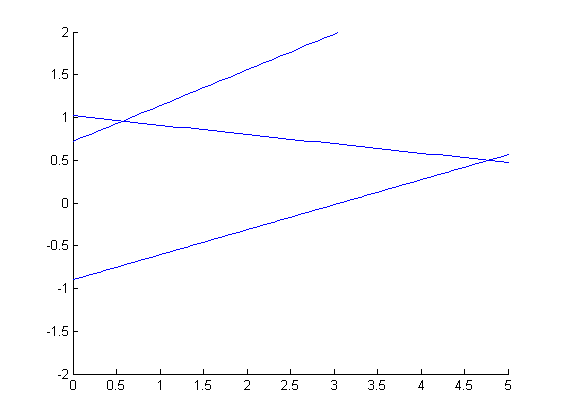
\includegraphics[width =0.7\textwidth]{ReF2013-2-1}
\caption{Opgave 2.1 -- tre versioner}
\label{fig:opg21}
\end{figure}

\begin{lstlisting}[caption=Matlab kode for Figur \ref{fig:opg21}, style=Code-Matlab, label=lst:21]
N = 3;

% A~U(-1,1)
A = rand(1,N)*2 - 1;
% A = [ -0.5 0 0.5 ];

% B~U(-2,2)
B = rand(1,N)*4 - 2;
% B = [ -1.5 0.1 1.4 ];

t = 0:0.1:5;

figure
hold on
for i = 1:N
    X = A(i)*t+B(i);
    plot(t,X)
end
axis([0 5 -2 2])
hold off
\end{lstlisting}
% subsection subsection_name (end)


\subsection*{2} % (fold)
\begin{align}
E\left[X(t) \right] &= E\left[A \cdot t + B\right] \\
	&= t \cdot E[A] + E[B] \\
	&= t \cdot 0 + 0 \\
	&= 0 \\
E \left[\left( X(t) \right)^2 \right] &= E \left[X(t) \cdot X(t) \right] \\
	&= E\left[(A \cdot t + B) \cdot (A \cdot t + B) \right] \\
	&= E\left[ (A \cdot t)^2 + (A \cdot t + B) \cdot 2 + B^2 \right] \\
	&= t^2 \cdot E\left[ A^2 \right] + 2t \cdot 2 \cdot E[A] + 2 \cdot E[B] + E\left[B^2 \right] \\
	&= t^2 \cdot Var(A) + 2 \cdot 0 + Var(B) \\
	&= t^2 \cdot \dfrac{\left( 1- (-1)\right)^2}{12} + \dfrac{\left( 2- (-2)\right)^2}{12} \\
	&= t^2 \cdot \dfrac{1}{3} + \dfrac{4}{3} & \text{Se Matlab herunder} \\
Var(X) &= E\left( X^2 \right) - \left( E[X] \right)^2 & E[X] = 0\\
	&= t^2 \cdot \dfrac{1}{3} + \dfrac{4}{3}
\end{align}

\begin{lstlisting}[caption=Opg 2.2, style=Code-Matlab, label=lst:Opg2.2]
syms t;
Var = t^2 * (1-(-1))^2/12 + (2-(-2))^2/12
\end{lstlisting}


% subsection 2 (end)

\subsection*{3} % (fold)
Autokorrelationsfunktion:
\begin{align}
R_X(t_1, t_2) &= E\left( X(t_1) \cdot X(t_2) \right) \\
	&=E\left[ (A \cdot t_1 + B) \cdot (A \cdot t_2 + B)\right] \\
	&=E\left[ A \cdot t_1 \cdot A \cdot t_2 + A \cdot t_1 \cdot B + A \cdot t_2 \cdot B + B^2 \right] \\
	&= t_1 \cdot t_2 \cdot E\left[ A^2\right] + t_1 \cdot E[A] \cdot E[B] + t_2 \cdot E[A] \cdot E[B] + E\left[B^2\right] \\
	&= t_1 \cdot t_2 \cdot Var(A) + t_1 \cdot 0 \cdot 0 + t_2 \cdot 0 \cdot 0 + Var(B) \\
	&= t_1 \cdot t_2 \cdot \frac{1}{3} +  \dfrac{4}{3} 
\end{align}
Processen er stationær hvis:
\begin{enumerate}
	\item $E\left( X(t) \right) = 0$, altså uafhængig af t.
	\subitem Det er den
	\item $R_X(t_1, t_2)$ er en funktion af $t_1-t_2$.
	\subitem Det er den ikke
\end{enumerate}
Den er derfor ikke stationær.
% section 3 (end)


% section opgave_2 (end)

\section*{Opgave 3} % (fold)
\label{sec:opgave_3}

\subsection*{1} % (fold)
Estimat af $\hat{\lambda}$:
\begin{align}
\hat{\lambda} &= \dfrac{x}{t} \\
	&= \dfrac{24}{3} \\
	&= 8
\end{align}

% subsection 1 (end)

\subsection*{2} % (fold)
\begin{align}
Pr\left(X > 6 \right) &= 1 - Pr(X \leq 6) \\
	&= 1- F_{posisson}(6)\\
	&= 0.6866 & \text{Se Matlab herunder}
\end{align}

\begin{lstlisting}[caption=Kode for Opg 3.2, style=Code-Matlab, label=lst:opg32]
x = 6;
lambda = 8;
Pr = 1-poisscdf(x, lambda)
\end{lstlisting}

% subsection 2 (end)

% section opgave_3 (end)

\newpage
\section*{Opgave 4} % (fold)
\label{sec:opgave_4}



% section opgave_4 (end)
\end{document}